\section{Código en \texttt{Python}}\label{apendice:tb_codigo}

Los programas que se presentan en esta sección contienen todo lo necesario para realizar todos los cálculos y gráficas a los que se ha hecho referencia en las secciones anteriores; están escritos en lenguaje de programación \texttt{Python 3.6.0} y se requiere tener instaladas las librerías \texttt{scipy 0.18}, \texttt{matplotlib 2.0.0}, \texttt{numpy 1.11.3} y \texttt{astropy 1.3}.
El código se encuentra repartido en varios ficheros llamados módulos. Para que los ejecutables funcionen correctamente, sin cambiar nada, debemos mantener la siguiente estructura de directorios: 

\hspace{3mm}

\begin{tikzpicture}[
    scale=.7,
    grow via three points={one child at (0.5,-0.65) and
    two children at (0.5,-0.65) and (0.5,-1.1)},
    edge from parent path={(\tikzparentnode.south) |- (\tikzchildnode.west)}]
  \node [root] {dir}
    child { node [selected] {packages}
        child { node {factor\_bayes.py}}
        child { node {get.py}}
        child { node {rojo.py}}
    }
    child { node at (0,-2)[selected] {p1\_halos}
        child { node [selected] {inroute}
            child { node {tabla\_Gonzalez-Nuevo\_2012.fits}}
            child { node {SMM\_template\_norm.sed}}
        }
        child { node at (0,-1.3)[selected] {outroute}}
        child { node at (0,-1.4){main\_halos.py}}
    }       
    child { node at (13,-1)[selected] {p2\_matching}
        child { node [selected] {inroute}
            child { node {GamaCoreDR1\_v1.fits}}
            child { node { HATLAS\_DR1\_CATALOGUE\_V1.2.FITS}}
            child { node { nombres\_candidatos.txt}}
            child { node { SMM\_template\_norm.sed}}
        }
        child { node at (0,-2.4)[selected] {outroute\_gama}}
        child { node at (0,-2.5)[selected] {outroute\_hatlas}}
        child { node at (0,-2.6)[selected] {outroute\_matching}}
        child { node at (0,-2.7){main\_gama.py}}
        child { node at (0,-2.8){main\_hatlas.py}}
        child { node at (0,-2.9){main\_matching\_gh.py}}
        child { node at (0,-3){main\_matching\_gh\_simulacion.py}}
    }
    child { node at (0,-5.1)[selected] {figuras\_adicionales}
        child { node [selected] {inroute}
            child { node {SMM\_template\_norm.sed}}
        }
        child { node at (0,-0.7)[selected] {outroute}}
        child { node at (0,-0.8){main\_ajuste\_error\_espec.py}}
        child { node at (0,-0.9){main\_radio\_Einstein\_D\_L.py}}
        child { node at (0,-1){main\_smm.py}}
    };
\end{tikzpicture}

\hspace{3mm}

Los ejecutables son todos aquellos ficheros cuyo nombre contiene la palabra \texttt{main}. Todos ellos leen los datos que necesitan de los ficheros situados en los directorios \texttt{inroute}, a excepción de los ejecutables \texttt{main\_matching.py} y \texttt{main\_matching\_simulacion.py} cuyos ficheros de entrada se encuentran en \texttt{outroute\_gama} y \texttt{outroute\_hatlas}. Las gráficas y tablas de datos se guardan en los directorios que contienen la palabra \texttt{outroute}. 

Todos los ejecutables hacen llamadas a una serie de funciones que son comunes, por ese motivo, para evitar repetir el código de esas funciones en cada ejecutable, éstas funciones se han definido en tres módulos que se encuentran el directorio \texttt{packages}. Cada módulo y cada función se encuentra debidamente comentada. Recuerdo al lector las cadenas de documentación son accesibles mediante:

\vspace{-2mm}

\begin{minted}{python}
    >>> help("nombre_modulo.nombre_funcion")
\end{minted}

\vspace{-4mm}

o

\vspace{-4mm}

\begin{minted}{python}
    >>> print(nombre_funcion.__doc__)
\end{minted}

\vspace{-2mm}

También se ha realizado un esquema sobre la estructura del ejecutable \texttt{main\_halos.py} (\ref{apendice:esquema_main_halos}). 

\let\thefootnote\relax\footnotetext{El código fuente de los programas escritos en \texttt{Python} y el escrito en \LaTeX\ con el que se obtiene este documento, están bajo licencia GPL.}

\newpage

\subsection{Esquema del módulo \texttt{main\_halos.py}}\label{apendice:esquema_main_halos}

\begin{figure}[!htp]
    \begin{center}
         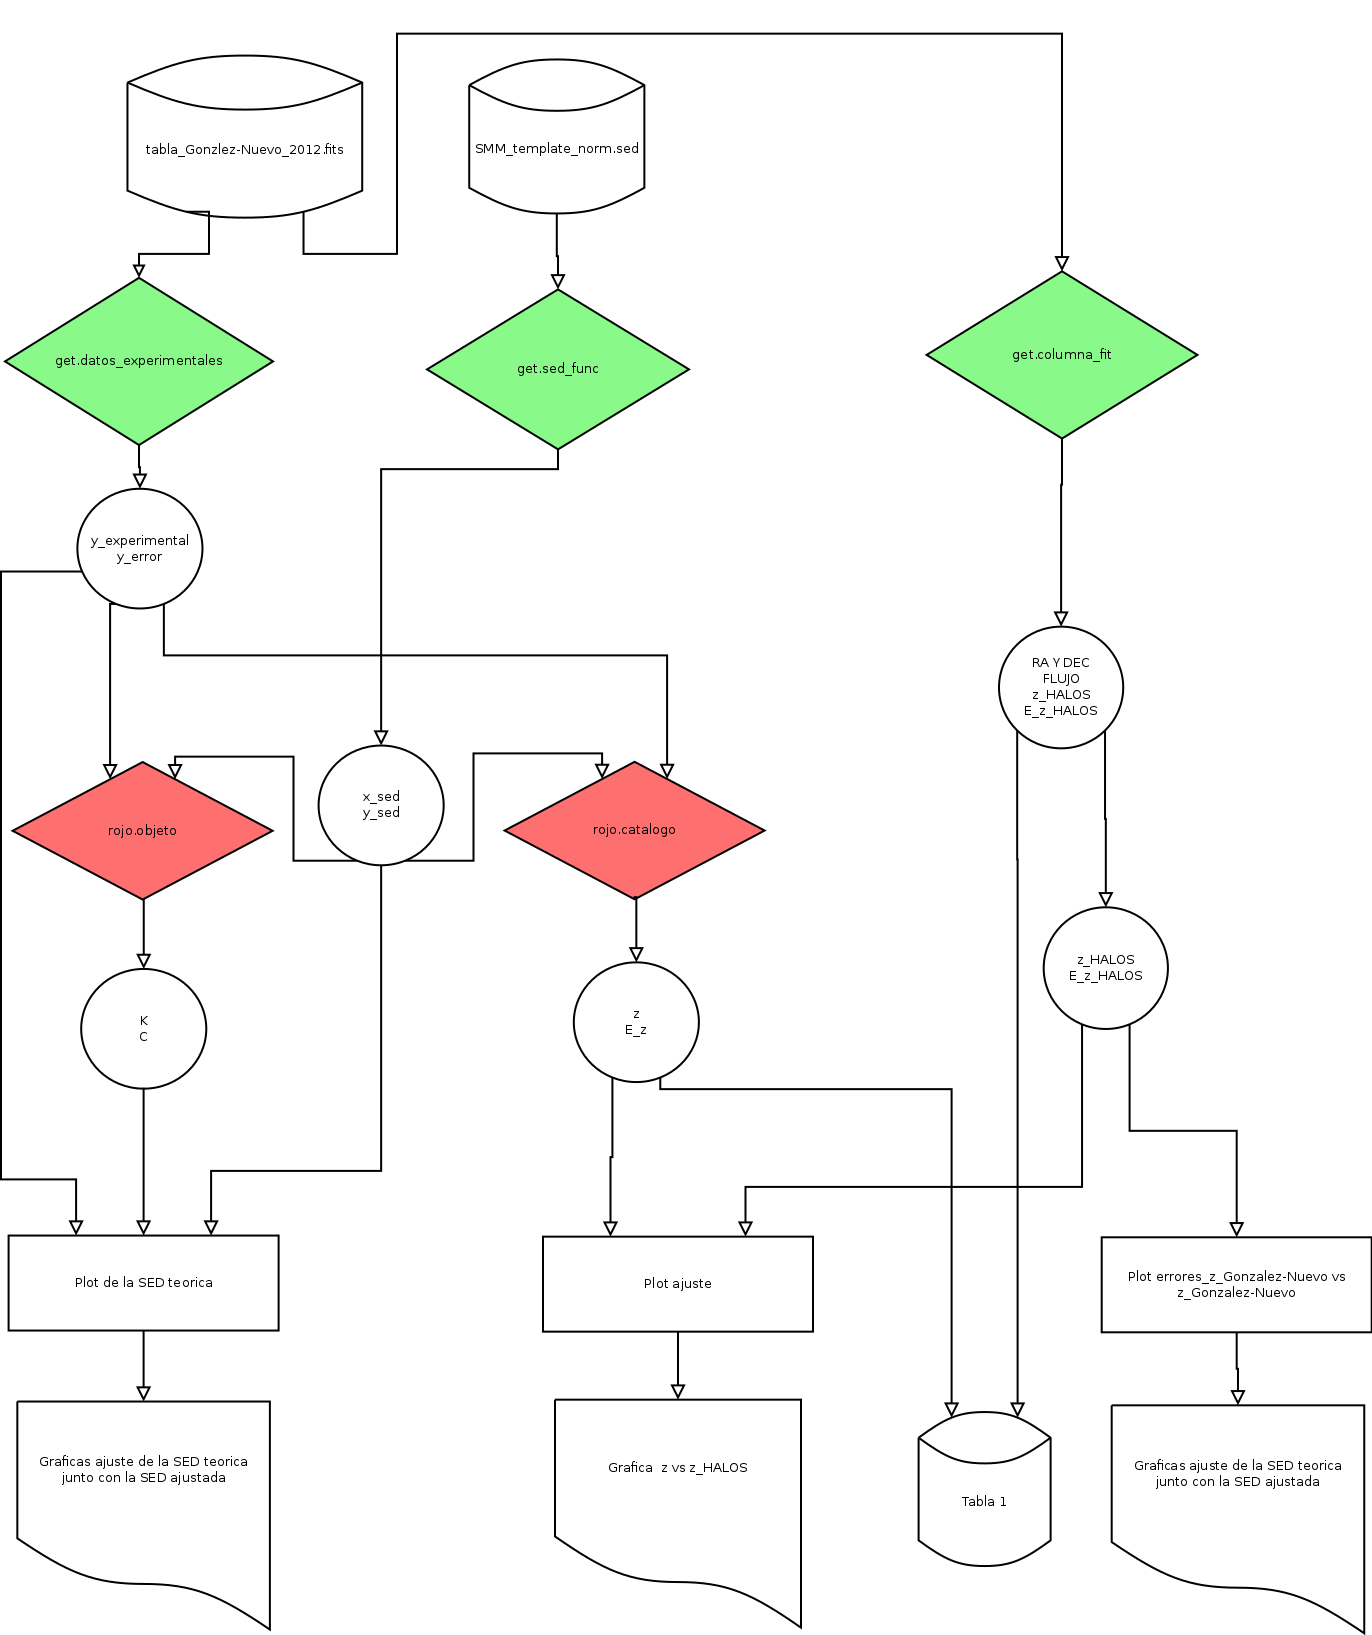
\includegraphics[width=16cm]{Apendices/codigo/Diagrama_p1.png}
    \end{center}
    \vspace{-3mm}
    \caption{Este esquema representa la estructura completa del ejecutable \texttt{main\_halos.py}. Los ficheros con formato \texttt{.fits} están representados mediante figuras cilíndricas; los que se encuentran en la parte superior de la figura, son los ficheros de entrada y el situado en la parte inferior es el fichero de salida a partir del cual se obtiene la tabla \ref{tab:redshift_halos}. Este ejecutable también devuelve varias figuras representadas en la zona inferior del esquema. Las funciones se representan mediante rombos y los colores ayudan a identificar el módulo en el que están definidas. La salida de que se obtiene a partir de cada función se encuentra en el interior de un círculo. }  
    \label{diagrama_flujo_main_halos}
\end{figure}

\newpage


\subsection{Módulo \texttt{main\_halos.py}}\label{apendice:codigo:main_halos}

\inputminted{python}{Apendices/codigo/main_halos.py}


\subsection{Módulo \texttt{main\_gama.py}}\label{apendice:codigo:main_gama}

\inputminted{python}{Apendices/codigo/main_gama.py}


\subsection{Módulo \texttt{main\_hatlas.py}}\label{apendice:codigo:main_hatlas}

\inputminted{python}{Apendices/codigo/main_hatlas.py}


\subsection{Módulo \texttt{main\_matching\_gh.py}}\label{apendice:codigo:main_matching_gh}

\inputminted{python}{Apendices/codigo/main_matching_gh.py}


\subsection{Módulo \texttt{main\_matching\_gh\_simulacion.py}}\label{apendice:codigo:main_matching_gh_simulacion}

\inputminted{python}{Apendices/codigo/main_matching_gh_simulacion.py}


\subsection{Módulo \texttt{factor\_bayes.py}}\label{apendice:codigo:factor_bayes}

\inputminted{python}{Apendices/codigo/factor_bayes.py}


\subsection{Módulo \texttt{rojo.py}}\label{apendice:codigo:rojo}

\inputminted{python}{Apendices/codigo/rojo.py}


\subsection{Módulo \texttt{get.py}}\label{apendice:codigo:get}

\inputminted{python}{Apendices/codigo/get.py}


\subsection{Módulo \texttt{main\_smm.py}}\label{apendice:codigo:main_smm}

\inputminted{python}{Apendices/codigo/main_smm.py}


\subsection{Módulo \texttt{main\_main\_radio\_Einstein\_D\_L.py}}\label{apendice:codigo:main_radio_Einstein_D_L}

\inputminted{python}{Apendices/codigo/main_radio_Einstein_D_L.py}


\subsection{Módulo \texttt{main\_ajuste\_error\_espec.py}}\label{apendice:codigo:main_ajuste_error_espec}

\inputminted{python}{Apendices/codigo/main_ajuste_error_espec.py}